We use four public datasets, two for \lda, \nytimes and \pubmed~\footnote{\url{http://archive.ics.uci.edu/ml/datasets/Bag+of+Words}}, 
and one each for \dl and \mmsb, \imagenet\footnote{\url{http://www.image-net.org/challenges/LSVRC/2010/download-public}} and 
\twitter\footnote{\url{http://konect.uni-koblenz.de/networks/twitter}} respectively.
\paragraph{\nytimes} It is a collection of news articles 



We compare our \method to \psgd (data partition), \dsgd (sync barrier) and \graphlab over scalability, 
   speed of convergence and convergence quality. \method performs best among all four approaches discussed 
   over all three application sets and evaluation criteria.  

\begin{figure}
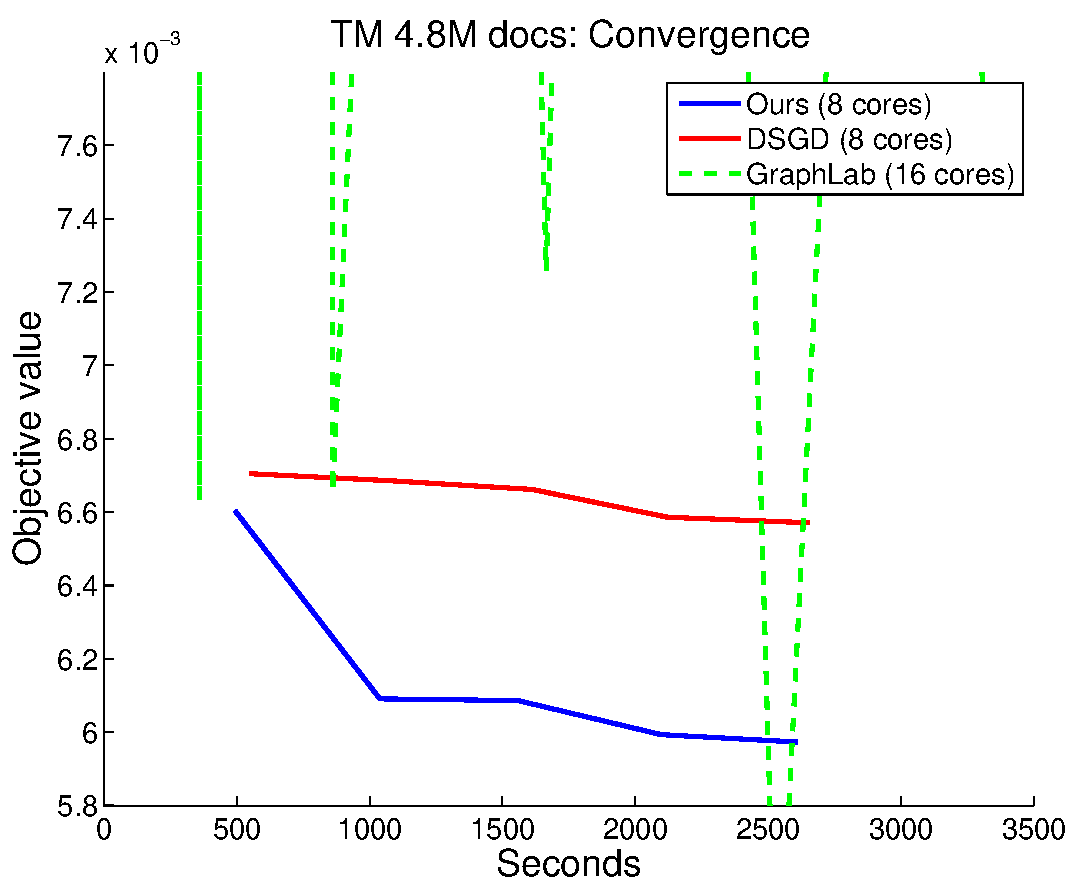
\includegraphics[width=0.23\textwidth]{results/tm_cvg.pdf} 
\label{fig:convergenceNytimes4}
\end{figure}



\begin{figure*}[t]
\centering
\begin{tabular}{|c|c|c|c|}
\hline
\multicolumn{4}{|c|}{\bf Topic Modeling} \\
\hline
Convergence Plots & \# of Topics & \# of Processors & \# of Docs \\
\hline
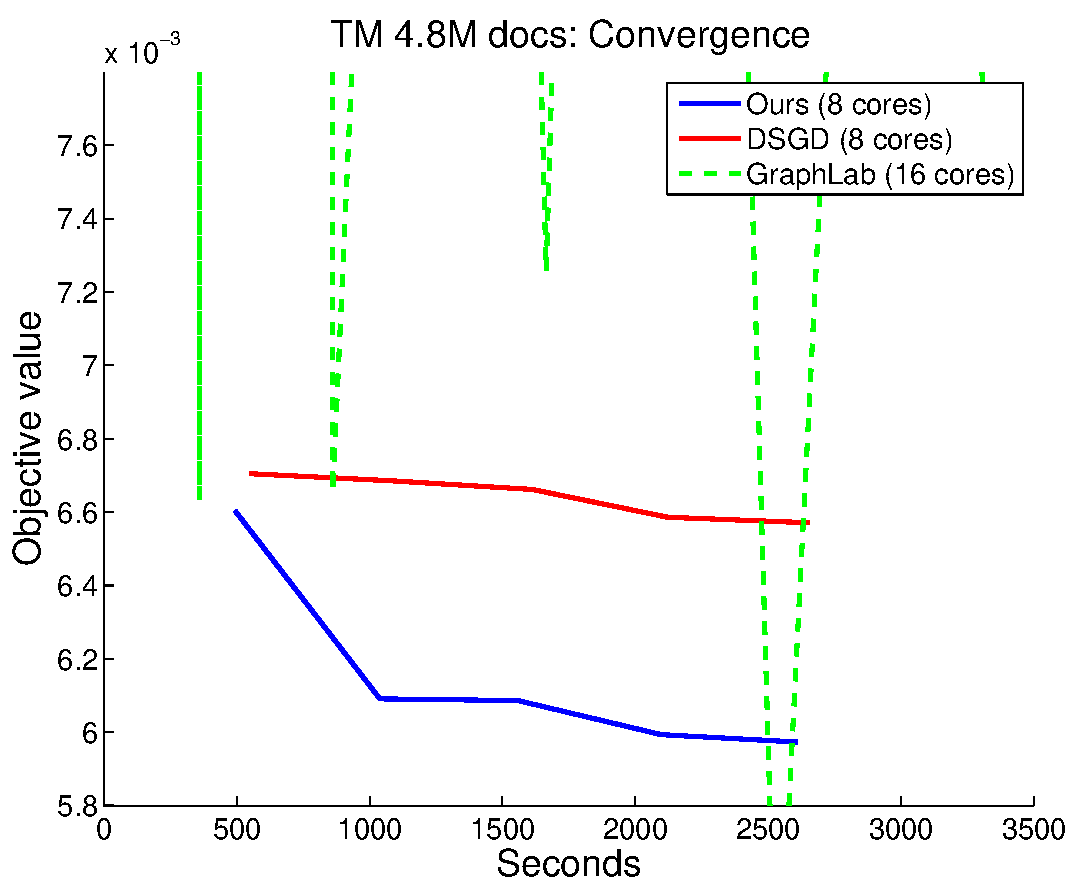
\includegraphics[width=0.23\textwidth]{results/tm_cvg.pdf} &
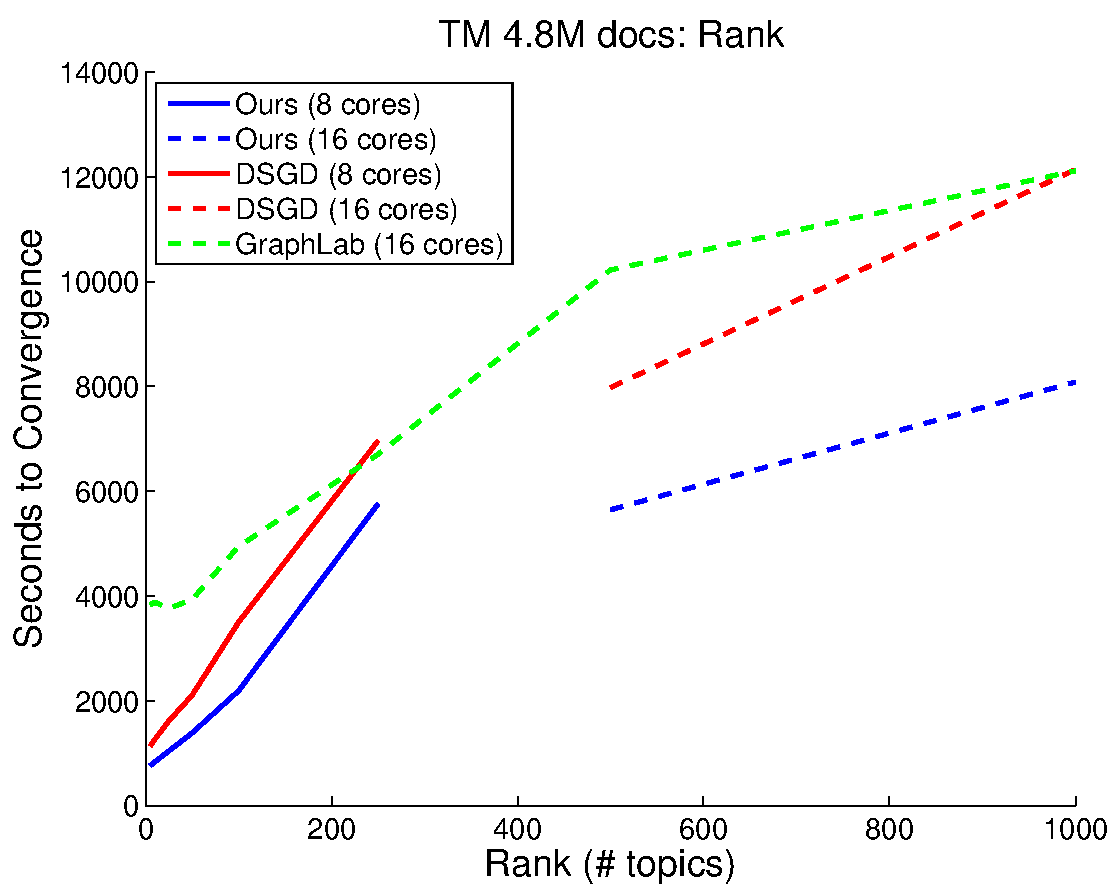
\includegraphics[width=0.23\textwidth]{results/tm_rank.pdf} &
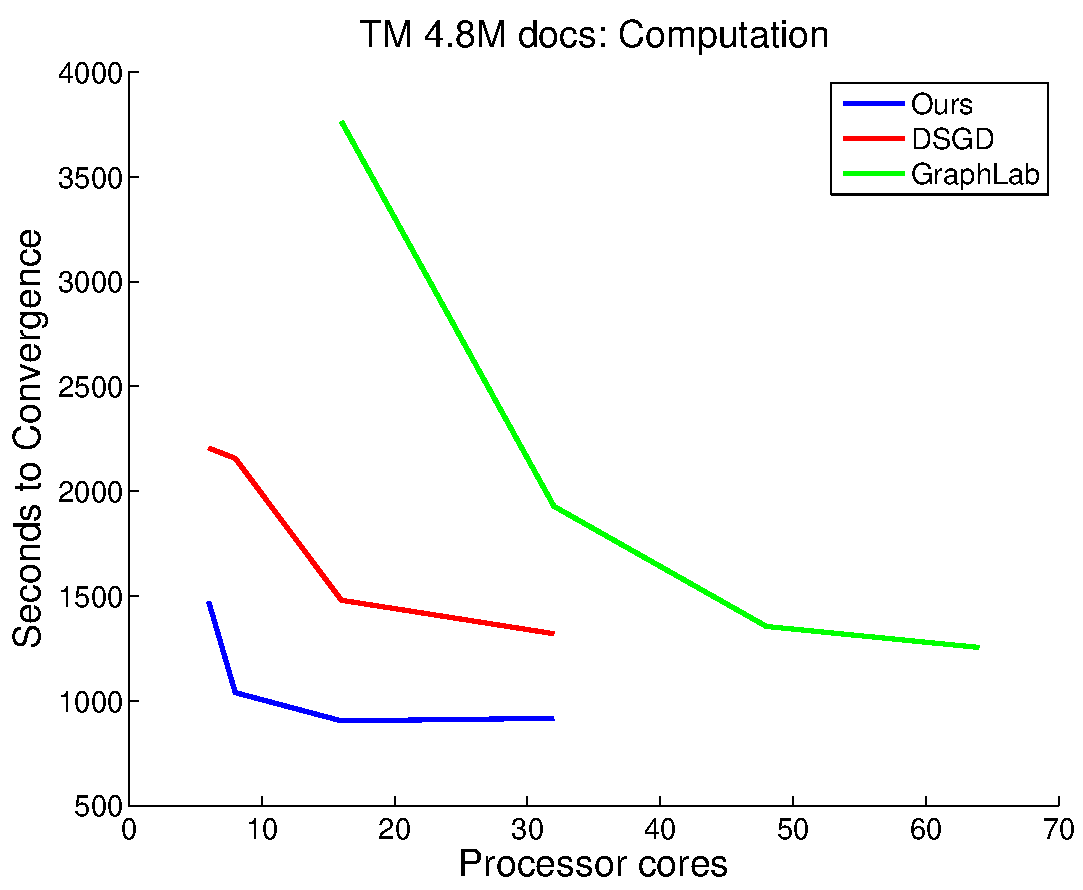
\includegraphics[width=0.23\textwidth]{results/tm_cores.pdf} &
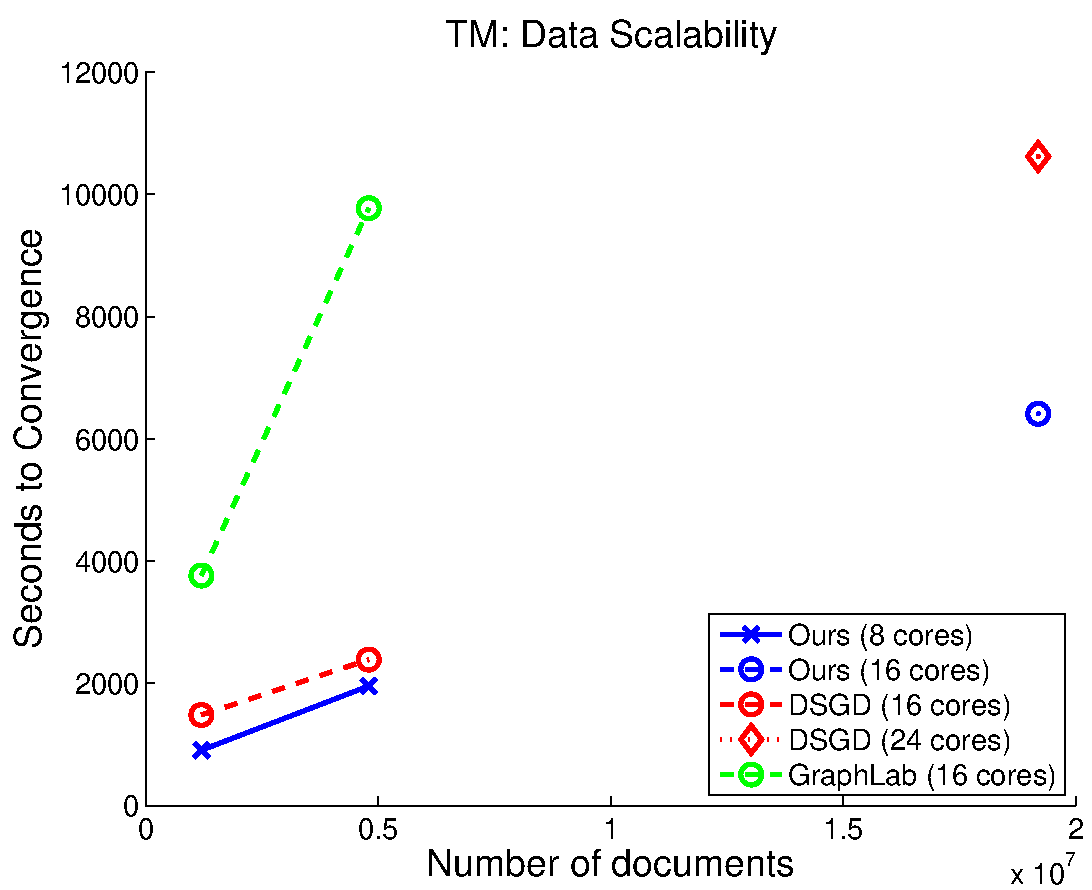
\includegraphics[width=0.23\textwidth]{results/tm_data.pdf} \\
\hline
\multicolumn{4}{|c|}{\bf Dictionary Learning} \\
\hline
Convergence Plots & \# of Dictionary Bases & \# of Processors & \# of Images \\
\hline
TODO&&&\\
\hline
\multicolumn{4}{|c|}{\bf Mixed Membership Network Decomposition} \\
\hline
Convergence Plots & \# of Network Roles & \# of Processors & \# of Network Nodes \\
\hline
TODO&&&\\
\hline
\end{tabular}
\caption{\small Convergence (Left) and scalability (in rank, processor cores and data size)
of all methods, on topic modeling, dictionary learning and mixed-membership network decomposition.
The convergence plot reveals the solution trajectory of each method, revealing pathological behavior such as oscillation.
The scalability plots show how each method fares as the problem rank, number of processor cores, and data
size is increased.}
\label{fig:results}
\end{figure*}
